% =============================================================================
% Lecture 13b: Model Serving, Part 2: Serving a Stream of Tokens
% Introduction to Machine Learning Systems (Volume I), Chapter 13
% =============================================================================
% Thesis: a language-model server meets two deadlines from one memory: decode
% bandwidth sets the floor of every token, the KV cache sets how many
% conversations share each weight read, and the scheduler decides who waits.
% Hook and synthesis: one 8x H100 server, Llama 2 70B, MLPerf Inference v5.0.
%
% Build: make -C slides build-13b_model_serving   (figures: images/make_figs.py)
% Plan:  lecture_map.yml in this folder.
% Numbers: the rendered chapter and cited papers; derived values say so.
% =============================================================================

\documentclass[aspectratio=169, 12pt]{beamer}
\usepackage{../../assets/beamerthememlsys}
\mlsyssetup{
  volume={Volume I},
  chapter={Chapter 13},
  chaptertitle={Model Serving, Part 2},
  layer=serving,
  logo={../../assets/img/logo-mlsysbook.png},
  instlogo={../../assets/img/logo-harvard.png},
  dividerstack,
}
\usepackage[T1]{fontenc}
\usepackage[scaled=0.9]{helvet}
\usepackage{courier}
\renewcommand{\familydefault}{\sfdefault}
\usepackage{booktabs,amsmath}
\usetikzlibrary{arrows.meta,positioning}
\graphicspath{{images/}}
% Generated by calcs.py. Do not edit; edit calcs.py and rerun it.
\defval{llama_off}{31{,}217}
\defval{llama_conv}{30{,}904}
\defval{llama_int}{12{,}979}
\defval{llama_int_off}{30{,}990}
\defval{llama_conv_ttft_s}{2}
\defval{llama_conv_tpot}{200}
\defval{llama_int_ttft}{450}
\defval{llama_int_tpot}{40}
\defval{llama_conv_pct}{99}
\defval{llama_int_pct}{42}
\defval{hook_answer}{40}
\defval{tpot_tighten}{5}
\defval{hook_fewer}{2.4}
\defval{mlperf_gpus}{8}
\defval{recall_b1_usd}{3.92}
\defval{recall_b8_usd}{0.52}
\defval{recall_ratio}{7.5}
\defval{recall_price}{4}
\defval{recall_rho_pct}{68}
\defval{recall_budget_ms}{50}
\defval{l3_kv_tok}{131{,}072}
\defval{l3_kv_kb}{131}
\defval{gpt2_params_b}{1.5}
\defval{gpt2_w_gb}{3}
\defval{gpt2_w_gb1}{3.0}
\defval{sw_h_ttft}{84}
\defval{sw_h_tbt}{28}
\defval{sw_h_e2e}{3{,}387}
\defval{sw_a_ttft}{155}
\defval{sw_a_tbt}{40}
\defval{sw_a_e2e}{4{,}957}
\defval{sw_decode_pct}{98}
\defval{sw_tokens}{120}
\defval{target_ttft}{500}
\defval{target_tpot}{50}
\defval{target_rate}{20}
\defval{h100_tflops}{989}
\defval{h100_bw}{3.35}
\defval{prefill_eff}{40}
\defval{gpt2_prompt}{512}
\defval{gpt2_prefill_tflop}{1.5}
\defval{gpt2_prefill_ms}{3.9}
\defval{cs_prompt}{1{,}000}
\defval{cs_ttft}{41.9}
\defval{gpt2_floor_ms}{0.9}
\defval{cs_w_gb}{4}
\defval{cs_floor_ms}{1.2}
\defval{cs_tpot_ms}{1.57}
\defval{cs_tpot_target}{20}
\defval{cs_room_ms}{18.4}
\defval{sw_prompt}{1{,}500}
\defval{sw_equiv}{6}
\defval{eager_ms}{8.6}
\defval{eager_kernels}{576}
\defval{decode_intensity}{1}
\defval{h100_ridge}{295}
\defval{spec_k}{4}
\defval{spec_k1}{5}
\defval{spec_alpha}{0.7}
\defval{spec_one_minus}{0.3}
\defval{spec_draft_ms}{0.296}
\defval{spec_verify_ms}{0.896}
\defval{spec_round_ms}{1.192}
\defval{spec_tokens}{2.8}
\defval{spec_per_token}{0.43}
\defval{spec_gain}{2.1}
\defval{spec_wrong}{3.8}
\defval{spec_draft_mb}{248}
\defval{lev_low}{2}
\defval{lev_high}{3}
\defval{gpt2_kv_kb}{307.2}
\defval{gpt2_kv_seq_gb}{0.31}
\defval{gpt2_kv_seq_gb4}{0.3146}
\defval{gpt2_ctx}{1{,}024}
\defval{step_gb_1}{3.3}
\defval{step_ms_1}{1.0}
\defval{rate_1}{1{,}011}
\defval{step_gb_32}{13.1}
\defval{step_ms_32}{3.9}
\defval{rate_32}{8{,}204}
\defval{batch_8}{8}
\defval{batch_32}{32}
\defval{batch_128}{128}
\defval{cache_share_32}{77}
\defval{tpot_growth}{3.9}
\defval{tpot_growth_0}{4}
\defval{rate_growth}{8.1}
\defval{step_ms_128}{12.9}
\defval{ceiling}{10{,}649}
\defval{b_tpot}{203}
\defval{b_mem}{263}
\defval{h100_mem_gb}{85.9}
\defval{h100_mem_gib}{80}
\defval{sw_batch}{64}
\defval{vb_short_in}{213}
\defval{vb_short_out}{512}
\defval{vb_long_in}{1{,}022}
\defval{vb_long_out}{128}
\defval{vb_conc}{64}
\defval{vb_ttft_med}{276}
\defval{vb_tpot}{9.50}
\defval{vb_tpot_1}{9.5}
\defval{vb_little}{6{,}737}
\defval{vb_rate}{6{,}411}
\defval{vb_share}{95}
\defval{vb_itl_p99_short}{12.55}
\defval{vb_itl_med_long}{11.13}
\defval{vb_itl_p99_long}{198.59}
\defval{vb_itl_ratio}{17.8}
\defval{len_a}{10}
\defval{len_b}{100}
\defval{len_c}{40}
\defval{len_d}{60}
\defval{len_e}{30}
\defval{req_end_e}{130}
\defval{req_end_f}{150}
\defval{req_end_g}{120}
\defval{req_end_h}{140}
\defval{cb_end_d}{60}
\defval{cb_end_e}{40}
\defval{cb_end_g}{60}
\defval{slots}{four}
\defval{a_idle}{90}
\defval{a_idle_pct}{90}
\defval{first_used}{210}
\defval{first_total}{400}
\defval{all_used}{350}
\defval{req_total}{600}
\defval{req_steps}{150}
\defval{req_util}{58}
\defval{cb_total}{400}
\defval{cb_steps}{100}
\defval{cb_util}{87.5}
\defval{e_wait}{100}
\defval{orca_gain}{36.9}
\defval{vllm_rate_low}{1.7}
\defval{vllm_rate_high}{2.7}
\defval{vllm_rate_ft}{22}
\defval{st_decodes}{32}
\defval{st_ctx}{1{,}256}
\defval{st_bytes}{9.3}
\defval{st_dec_ms}{2.8}
\defval{st_stall_ms}{44.7}
\defval{st_chunks}{four}
\defval{st_chunk_tok}{250}
\defval{st_chunk_pre}{10.5}
\defval{st_chunk_ms}{13.3}
\defval{st_first}{53}
\defval{st_safe}{411}
\defval{sarathi_low}{2.6}
\defval{sarathi_high}{3.7}
\defval{l3_w16_gb}{16.1}
\defval{conv_tokens}{8{,}192}
\defval{conv_gb}{1.07}
\defval{free_gb}{69.8}
\defval{n_conv}{65}
\defval{n_conv_noweights}{80}
\defval{n_conv_gb}{69.8}
\defval{kv70_budget}{50.6}
\defval{kv70_tok}{327{,}680}
\defval{kv70_ratio}{2.5}
\defval{kv70_batch}{32}
\defval{kv70_cross}{4{,}800}
\defval{kv70_layers}{80}
\defval{kv70_heads}{8}
\defval{kv70_hdim}{128}
\defval{kwon_param_pct}{65}
\defval{kwon_kv_pct}{30}
\defval{orca_used_low}{20.4}
\defval{orca_used_high}{38.2}
\defval{vllm_used}{96.3}
\defval{vllm_batch_orca}{13.6}
\defval{vllm_batch_vllm}{30.4}
\defval{vllm_batch_gain}{2.2}
\defval{block_default}{16}
\defval{log_weights_gib}{14.96}
\defval{log_weights_gb}{16.1}
\defval{log_tokens}{420{,}976}
\defval{log_kv_gib}{51.39}
\defval{log_conc}{51.39}
\defval{log_conc_0}{51}
\defval{log_util}{0.9}
\defval{log_util_pct}{90}
\defval{log_claimed_gib}{72}
\defval{log_workspace_gib}{5.65}
\defval{log_high_pct}{26}
\defval{log_req_tokens}{1{,}256}
\defval{log_blocks}{79}
\defval{log_paged_est}{421}
\defval{log_paged_pool}{333}
\defval{cs_resident}{469}
\defval{block_waste_mb}{2}
\defval{prefix_tokens}{2{,}000}
\defval{prefix_mb}{262}
\defval{prefix_users}{100}
\defval{prefix_saved_gb}{26}
\defval{prefix_copies_gb}{26.2}
\defval{prefix_shared_gb}{0.26}
\defval{prefix_users_less1}{99}
\defval{reload_ms}{34}
\defval{reload_gbps}{32}
\defval{share_ps_low}{6.1}
\defval{share_ps_high}{9.8}
\defval{share_bs_low}{37.6}
\defval{share_bs_high}{55.2}
\defval{ds_colo}{1.6}
\defval{ds_pre}{5.6}
\defval{ds_dec}{10}
\defval{ds_params}{13}
\defval{ds_in}{512}
\defval{ds_out}{64}
\defval{ds_slo_pct}{90}
\defval{ds_pre_exact}{1.8}
\defval{ds_pre_n}{2}
\defval{ds_gpus}{3}
\defval{ds_gpus_word}{three}
\defval{ds_per_gpu}{3.3}
\defval{ds_gain}{2.1}
\defval{ds_more}{7.4}
\defval{ds_tighter}{12.6}
\defval{ds_kv_gb}{1.13}
\defval{ds_kv_rate}{10}
\defval{ds_traffic}{11.3}
\defval{ds_traffic_gbps}{90}
\defval{ds_link}{600}
\defval{ds_xfer_pct}{0.1}
\defval{sw_xfer_pct}{0.8}
\defval{sw_xfer_ms}{5}
\defval{sw_cap_from}{700}
\defval{sw_cap_to}{350}
\defval{sw_gain}{1.4}
\defval{sw_cost_pct}{20}
\defval{p_node}{1{,}000}
\defval{p_node_kw}{1}
\defval{p_low}{600}
\defval{p_low_gpu}{300}
\defval{p_host}{300}
\defval{j1}{0.99}
\defval{j32}{0.12}
\defval{j1_low}{0.59}
\defval{j_low_ratio}{4.9}
\defval{p_ratio}{1.7}
\defval{cc_joules}{1.1}
\defval{cc_low_joules}{6.6}
\defval{g_reduction}{33}
\defval{g_model}{23}
\defval{g_util}{1.4}
\defval{g_wh}{0.24}
\defval{cs_price}{3}
\defval{cs_prefill_rate}{10{,}000}
\defval{cs_req_rate}{10}
\defval{cs_decode}{256}
\defval{cs_tokens}{1{,}256}
\defval{cs_mtok_h}{45.2}
\defval{cs_usd_m}{0.066}
\defval{price_gpt4}{30}
\defval{price_flash}{0.075}
\defval{llama_conv_tpot_s}{0.2}
\defval{llama_int_tpot_s}{0.04}
\defval{streams_200}{6{,}181}
\defval{streams_40}{519}
\defval{syn_mem_gb}{687}
\defval{syn_w16_gb}{141}
\defval{syn_w4_gb}{35.3}
\defval{syn_w_ratio}{4}
\defval{syn_free_gb}{546}
\defval{syn_conv_mb}{412}
\defval{syn_streams}{1{,}326}
\defval{syn_step_ms}{43}
\defval{syn8_free_gb}{617}
\defval{syn8_conv_mb}{206}
\defval{syn8_streams}{3{,}000}
\defval{syn_servers}{2.4}

% The figures' compute (orange) and memory (blue) colors, for text beside them
\definecolor{figcompute}{HTML}{E67817}
\definecolor{figmemory}{HTML}{006395}
\setcounter{mlsystotalsections}{5}

\title{Model Serving, Part 2}
\author{Vijay Janapa Reddi}
\institute{Harvard University}
\date{}

% A large answer choice for predict and concept-question slides
\newcommand{\choice}[2]{\textbf{\textcolor{mlsysaccent}{#1}}\enspace #2}
% A choice that is highlighted from overlay #1 on (the answer)
\newcommand{\answerat}[3]{\alt<#1->{\colorbox{mlsysaccent!15}{\choice{#2}{#3}}}{\choice{#2}{#3}}}
% A goal or takeaway line with its thumbnail
\newcommand{\thumbline}[2]{%
  \begin{minipage}[c]{2.6cm}\centering\includegraphics[width=2.5cm,height=0.95cm,keepaspectratio]{#1}\end{minipage}%
  \hspace{0.3cm}\begin{minipage}[c]{0.74\textwidth}\small #2\end{minipage}}
% One line of a worked example: shown from overlay #1 on
\newcommand{\wstep}[2]{\uncover<#1->{#2}\\[0.22cm]}
% An exact excerpt of real tool output or source code, at a legible size
\newenvironment{logblock}[1][7]{\par\ttfamily\fontsize{#1}{8.3}\selectfont\raggedright\setlength{\parskip}{0pt}}{\par}
% One aligned "label: value" row of a tool's printed table (alignment spaces become \hfill)
\newcommand{\logrow}[2]{\makebox[\linewidth][l]{#1\hfill #2}\\}
% Code indentation of n spaces in the current monospace font
\newcommand{\ind}[1]{\hspace*{#1\fontcharwd\font`0}}


\begin{document}

% =============================================================================
% TITLE AND HOOK
% =============================================================================
\mlsysnote{[0.5 min] [CORE] Read the thesis aloud once. Part 1 served one fixed-size answer per request: a budget, a queue, a batch, a replica. Today the answer is a stream of hundreds of tokens, and each conversation holds memory until it ends. The notes total about 72 minutes. FLEX: notes tagged [OPTIONAL] can be cut; cutting all of them leaves a complete lecture of about 49.5 minutes. Cut first the joules slide and the open questions.}
\mlsystitle{Model Serving, Part~2}{In a stream of tokens, every token costs a weight read, and the KV cache sets how many conversations share it.}{cover_model_serving_blueprint.png}

\begin{frame}{Predict: what does a tighter token deadline cost?}
  \mlsysactivity{Predict}{2 min}
  \centering
  \mlsyssteps[width=0.92\textwidth,height=4.6cm,keepaspectratio]{hook_step}{4}\\[0.02cm]
  {\footnotesize\textcolor{midgray}{TTFT: time to first token.\quad TPOT: time per output token.}}\\[0.1cm]
  {\normalsize\choice{A}{about the same}\qquad\choice{B}{about 80\%}\qquad\answerat{4}{C}{about \val{hook_answer}\%}\qquad\choice{D}{about 10\%}}
  \mlsyscredit{MLPerf Inference v5.0, closed, datacenter, Dell PowerEdge XE9680, \val{mlperf_gpus}$\times$ H100-SXM-80GB (5.0-0020): Llama 2 70B Offline, Server, and interactive Server. Bounds: v5.0 inference rules.}
  \note{[3 min] [CORE] One server with eight H100s, one model, Llama 2 70B, measured in MLPerf. Step 1: with no deadline (Offline), \val{llama_off} tokens per second. Step 2: the Server scenario with random arrivals and two deadlines: the first token within \val{llama_conv_ttft_s} s (TTFT, time to first token) and a time per output token (TPOT), each request's average gap between the tokens that follow, of at most \val{llama_conv_tpot} ms. MLPerf checks both bounds at the Server scenario's 99th-percentile latency rule. The server keeps \val{llama_conv} tokens per second, \val{llama_conv_pct} percent. Step 3: the interactive bound tightens TPOT to \val{llama_int_tpot} ms and TTFT to \val{llama_int_ttft} ms. ENGAGE: students vote with fingers. Step 4: C. \val{llama_int} tokens per second, \val{llama_int_pct} percent of the conversational rate. Students who chose A reasoned that one token takes far less than \val{llama_int_tpot} ms, which is true at batch one; students who chose D scaled throughput with the deadline. WARN: the interactive run is a separate MLPerf benchmark entry with its own Offline run (\val{llama_int_off} tokens per second); the comparison is fair. LINK: Lecture 12 introduced MLPerf's Offline and Server scenarios; TTFT and TPOT are new today, and the next segment defines them on one request. Today explains the drop; the synthesis returns to these bars.}
\end{frame}

\begin{frame}{Recall: what sizes a fleet, and what does a batch cost?}
  \mlsysactivity{Retrieval}{1.5 min}
  \begin{columns}[c]
    \begin{column}{0.56\textwidth}
      {\Large\bfseries Question of the day}\\[0.2cm]
      {\normalsize Which three quantities size a serving fleet? What does a batch cost the request that waits for it?}\\[0.3cm]
      \uncover<2->{\small\textbf{\textcolor{mlsysaccent}{Service time}} per request\\
      \textbf{\textcolor{mlsysaccent}{Utilization}} the tail target allows\\
      \textbf{\textcolor{mlsysaccent}{Peak rate}} with headroom\\[0.1cm]
      A batch shares fixed costs; every request pays the wait to form it.}
    \end{column}
    \begin{column}{0.40\textwidth}
      \centering\safeimg[width=\textwidth,height=1.3cm,keepaspectratio]{thumb_recall_cost.pdf}\\[0.02cm]
      {\footnotesize ResNet-50: \$\val{recall_b1_usd} per million at batch 1, \$\val{recall_b8_usd} at batch \val{batch_8}}\\[0.15cm]
      \uncover<3->{\begin{mlsyscard}{mlsysaccent}\small\textbf{From Lecture 6b:} decode reads every weight for every token. Llama 3 8B keeps \textbf{\val{l3_kv_kb} KB} of KV cache per token.\end{mlsyscard}}
    \end{column}
  \end{columns}
  \mlsyscredit{Lecture 13 (Part 1): Model Serving, Example 13.1 (modeled, \$\val{recall_price} per GPU-hour). Lecture 6b; \val{l3_kv_tok} B per token: Model Serving, \S13.9.5.}
  \note{[1.5 min] [CORE] Retrieval from Part 1. Give 45 seconds. Step 2: service time per request; the highest utilization the tail target allows (about \val{recall_rho_pct} percent for Part 1's \val{recall_budget_ms} ms budget); the peak rate with headroom. A batch shares the fixed cost of a pass, which is why batch \val{batch_8} cost \val{recall_ratio} times less than batch 1 in the thumbnail, but each request waits for the batch to form. Step 3: one line from Lecture 6b, given without a second derivation. Each decode step reads every weight to produce one token, and each token of context keeps a key and a value in every layer, the KV cache: \val{l3_kv_tok} bytes for Llama 3 8B in 16-bit precision. ENGAGE: what changes when one request is not one forward pass but hundreds, and holds memory the whole time? Take two answers; segments 1 to 3 answer it. FLEX: a student who missed Part 1 needs only this slide.}
\end{frame}

\begin{frame}{How does one GPU serve many chats, one token at a time?}
  \thumblinesm{thumb_ttft_step4.pdf}{Say which phase sets TTFT and which sets TPOT; compute the decode floor and a speculative-decoding gain.}\\[0.2cm]
  \thumblinesm{thumb_cb_step7.pdf}{Work a continuous-batching schedule, and find the largest batch a TPOT target allows.}\\[0.2cm]
  \thumblinesm{thumb_paging_step4.pdf}{Budget KV memory, and show how paging and sharing raise the conversations it holds.}\\[0.2cm]
  \thumblinesm{thumb_distserve_pool.pdf}{Decide when to split prefill and decode, and price a token in joules and dollars.}\\[0.3cm]
  {\footnotesize\textcolor{midgray}{Running models: GPT-2 XL and Llama 3 8B on one H100 (the chapter); Llama 2 70B on \val{mlperf_gpus}$\times$ H100 (MLPerf).}}\par\vspace{0.15cm}
  \threadstrip{0}{1}{0}{0}{1}
  \note{[1 min] [CORE] For the driving question, note that a chat answer is hundreds of tokens produced one at a time. How does one accelerator serve many conversations at once without breaking either deadline, and what does each token cost? Four goals, one per part of the lecture; each thumbnail is the shape of the figure that teaches it. Three models carry the numbers. GPT-2 XL (\val{gpt2_params_b} billion parameters, \val{gpt2_w_gb} GB in 16-bit) is the chapter's example of a bandwidth-bound decoder. Llama 3 8B is the chapter's case study. Llama 2 70B is the measured hook. The strip fills the machine factor of the iron law and the fast-enough half of the dual mandate.}
\end{frame}

% =============================================================================
% SECTION: TWO DEADLINES
% =============================================================================
\mlsysnote{[0.5 min] [CORE] First, one request on an idle server: which phase sets which deadline?}
\mlsysdivider{What sets the first token, and each next one?}{Model Serving, \S13.9.1, \S13.9.2, \S13.9.4}
\section{Deadlines}

\begin{frame}{A chat answer has two deadlines, the first token and each one after it}
  \centering
  \mlsyssteps[width=0.95\textwidth,height=5.8cm,keepaspectratio]{ttft_step}{4}
  \mlsyscredit{Patel et al., ``Splitwise,'' ISCA 2024, Table IV (Llama 2 70B, P50, no batching, conversation trace). Targets: Model Serving, Systems Perspective 13.5 (illustrative).}
  \note{[2.5 min] [CORE] Step 1: one measured chat request, Llama 2 70B on one eight-GPU DGX-H100, no batching, the median of a conversation trace. Prefill reads the whole prompt in parallel and produces the first token at \val{sw_h_ttft} ms: TTFT. Decode then produces one token every \val{sw_h_tbt} ms: TPOT, the average gap between tokens. The answer of about \val{sw_tokens} tokens ends at \val{sw_h_e2e} ms. Step 2: decode is \val{sw_decode_pct} percent of the request (our arithmetic from the two medians; the paper says most of the time). Step 3: the same request on the older DGX-A100: \val{sw_a_ttft} ms, then a token every \val{sw_a_tbt} ms, \val{sw_a_e2e} ms in all. Step 4: the chapter's illustrative targets: the first token within \val{target_ttft} ms, then a token every \val{target_tpot} ms, \val{target_rate} tokens per second, faster than people read. ENGAGE: which deadline does a user notice first, and which one decides whether the answer feels fast? WARN: a fast first token does not mean a fast answer; the two phases have different limits.}
\end{frame}

\begin{frame}{Prefill spends arithmetic; decode spends a weight read}
  \begin{columns}[c]
    \begin{column}{0.70\textwidth}
      \centering\mlsyssteps[width=\textwidth,height=5.0cm,keepaspectratio]{phases_step}{4}
    \end{column}
    \begin{column}{0.28\textwidth}
      \centering\mlsysphoto[width=\textwidth,height=2.4cm,keepaspectratio]{nvidia-h100-pcie.jpg}\\[0.08cm]
      {\footnotesize NVIDIA H100 (PCIe card shown). The chapter's H100 SXM:\\[0.04cm]
      \textbf{\textcolor{figcompute}{\val{h100_tflops} TFLOP/s}} FP16 for prefill\\
      \textbf{\textcolor{figmemory}{\val{h100_bw} TB/s}} HBM3 for decode}
    \end{column}
  \end{columns}
  \vspace{0.05cm}
  \centering\uncover<2->{\footnotesize Measured (Splitwise, BLOOM-176B): a \val{sw_prompt}-token prompt takes as long as \val{sw_equiv} output tokens.}
  \mlsyscredit{Model Serving, \S13.9.2 and \S13.10.3 (modeled). Patel et al., ``Splitwise,'' ISCA 2024, \S III-C. Photo: Geekerwan, CC BY 3.0, Wikimedia Commons.}
  \note{[3 min] [CORE] Point to the photo: one H100 has two ceilings, \val{h100_tflops} trillion 16-bit operations per second and \val{h100_bw} TB/s of memory bandwidth, and the two phases hit different ones. (The photo shows the PCIe card; the chapter's numbers are for the SXM module, the same chip with faster memory.) Step 1: prefill. GPT-2 XL's \val{gpt2_prompt}-token prompt is about \val{gpt2_prefill_tflop} TFLOP; at \val{prefill_eff} percent of the 16-bit peak it takes \val{gpt2_prefill_ms} ms. Llama 3 8B's \val{cs_prompt}-token prompt takes \val{cs_ttft} ms. Prefill grows with prompt length and sets TTFT. Step 2: decode reads every weight to make one token. GPT-2 XL's \val{gpt2_w_gb} GB at \val{h100_bw} TB/s cannot take less than \val{gpt2_floor_ms} ms; Llama 3 8B with 4-bit (INT4) weights reads \val{cs_w_gb} GB, a floor of \val{cs_floor_ms} ms, \val{cs_tpot_ms} ms with kernel-launch cost. Measured: \val{sw_prompt} prompt tokens cost as much time as \val{sw_equiv} output tokens. Step 3: issued kernel by kernel from Python, one GPT-2 XL step spends \val{eager_ms} ms launching \val{eager_kernels} kernels; servers replay the step as one CUDA graph. Step 4: in a \val{cs_tpot_target} ms TPOT, one step uses \val{cs_tpot_ms} ms; \val{cs_room_ms} ms is room to share this weight read. LINK: Lecture 6b placed decode at \val{decode_intensity} FLOP per byte against the ridge near \val{h100_ridge}; Lecture 7 owns graph capture; Lecture 10b owns INT4.}
\end{frame}

\begin{frame}{Estimate: tokens per speculative round}
  \mlsysactivity{Estimate}{2 min}
  \centering
  \mlsyssteps[width=0.95\textwidth,height=2.9cm,keepaspectratio]{spec_step}{2}\\[0.05cm]
  \begin{columns}[T]
    \begin{column}{0.40\textwidth}
      \begin{mlsyscard}{mlsysaccent}
        \small\textbf{Given: GPT-2 XL}\\[0.05cm]
        Draft: GPT-2 Small, $k = \val{spec_k}$\\
        Each draft token kept: $\alpha = \val{spec_alpha}$\\
        Round: \val{spec_draft_ms} + \val{spec_verify_ms} = \val{spec_round_ms} ms
      \end{mlsyscard}
    \end{column}
    \begin{column}{0.56\textwidth}
      \small
      \wstep{3}{Tokens per round $= \dfrac{1-\alpha^{k+1}}{1-\alpha} = \dfrac{1-\val{spec_alpha}^{\val{spec_k1}}}{\val{spec_one_minus}} = \mathbf{\val{spec_tokens}}$}
      \wstep{3}{$\val{spec_round_ms} / \val{spec_tokens} = \val{spec_per_token}$ ms per token, against \val{spec_verify_ms}: \textbf{\textcolor{mlsysaccent}{\val{spec_gain}$\times$}}}
      \uncover<3->{\footnotesize\textcolor{midgray}{Measured: \val{lev_low} to \val{lev_high}$\times$ on T5-XXL (Leviathan et al.).}}
    \end{column}
  \end{columns}
  \mlsyscredit{Model Serving, \S13.9.4 and equation 15 (acceptance assumed). Leviathan et al., ICML 2023.}
  \note{[2.5 min] Decode at batch one reads the weights for one token. Speculative decoding gets more than one token per read. Step 1: a small draft model, GPT-2 Small (\val{spec_draft_mb} MB), proposes \val{spec_k} tokens in \val{spec_draft_ms} ms. The target model then checks all \val{spec_k1} positions in one pass, about one weight read, \val{spec_verify_ms} ms, because checking known tokens is parallel, like prefill. Step 2: the target keeps the longest run of draft tokens it agrees with, plus one token of its own. In this round it kept two, rejected the third, dropped the fourth, and added its own: 3 tokens. ENGAGE: two minutes in pairs; how many tokens per round on average if each draft token is kept with probability \val{spec_alpha}? Step 3: equation 15 gives \val{spec_tokens}, so \val{spec_per_token} ms per token, \val{spec_gain} times faster. Students who answer \val{spec_k} forget rejections; students who answer \val{spec_wrong} add \val{spec_alpha} times \val{spec_k} to the target token without the rule that one rejection ends the run. WARN: the \val{spec_alpha} is assumed. The gain shrinks as acceptance falls, and at large batch the extra positions cost arithmetic a full batch no longer has spare. FLEX: [OPTIONAL]; cutting it loses speculative decoding.}
\end{frame}

% =============================================================================
% SECTION: SHARING THE STEP
% =============================================================================
\mlsysnote{[0.5 min] [CORE] Land the first segment aloud: prefill sets TTFT, decode sets TPOT, and at batch one a decode step uses a sliver of its deadline. Now spend the rest of the deadline on other conversations.}
\mlsysdivider{How many chats can share one decode step, and who waits?}{Model Serving, \S13.9.2 and \S13.9.4}
\section{Sharing}

\begin{frame}{Decode batches share weights; KV caches stay separate}
  \mlsysactivity{Predict}{1 min}
  \centering
  \mlsyssteps[width=0.95\textwidth,height=4.0cm,keepaspectratio]{decode_bytes_step}{2}\\[0.1cm]
  {\small GPT-2 XL, full \val{gpt2_ctx}-token contexts. From batch 1 to \val{batch_32}, each user's TPOT grows:}\\[0.15cm]
  {\normalsize\choice{A}{\val{batch_32}$\times$}\qquad\answerat{2}{B}{about \val{tpot_growth_0}$\times$}\qquad\choice{C}{not at all: the weights are shared}}
  \mlsyscredit{Model Serving, \S13.9.2 (modeled; \val{gpt2_kv_kb} KB of cache per token, no grouped-query sharing).}
  \note{[2.5 min] [CORE] The KV cache holds the keys and values of every earlier token, so a step need not recompute them. GPT-2 XL keeps \val{gpt2_kv_kb} KB per token, \val{gpt2_kv_seq_gb} GB for a full \val{gpt2_ctx}-token context. Step 1: batch 1. A step reads the \val{gpt2_w_gb} GB of weights and one cache: \val{step_gb_1} GB in \val{step_ms_1} ms, \val{rate_1} tokens per second. ENGAGE: one minute, vote. Step 2: B. At batch \val{batch_32} the weights are still read once, but every sequence reads its own cache: \val{step_gb_32} GB, \val{cache_share_32} percent of it cache, in \val{step_ms_32} ms. Each user waits \val{tpot_growth} times longer per token, and the server makes \val{rate_32} tokens per second, \val{rate_growth} times more. A treats the batch as \val{batch_32} separate requests; C is right only for the weight read. WARN: in Part 1 a ResNet-50 batch shared everything but the input; here every conversation brings its own growing state. LINK: Lecture 6b showed why grouped-query attention shrinks this cache; Llama 3 8B uses it, GPT-2 XL does not.}
\end{frame}

\begin{frame}{A TPOT target caps the batch, and memory caps it again}
  \centering
  \mlsyssteps[width=0.95\textwidth,height=4.9cm,keepaspectratio]{frontier_step}{3}\\[0.0cm]
  \uncover<3->{\footnotesize Measured (Splitwise, H100): a batch of \val{sw_batch} only doubles TPOT; then memory runs out.}
  \mlsyscredit{Model Serving, \S13.9.2 (batch 1 and \val{batch_32}) and \S13.9.5 (\val{h100_mem_gb} GB, the H100's \val{h100_mem_gib} GiB in decimal units). Gray points derived: (\val{gpt2_w_gb1} + \val{gpt2_kv_seq_gb4} B) GB / \val{h100_bw} TB/s. Patel et al., ``Splitwise,'' \S III-C, Fig.~6b.}
  \note{[2.5 min] [CORE] Each point is one batch size. Across: tokens per second for the whole server. Up: each user's time per token. Step 1: the book's two points, batch 1 and \val{batch_32}, and batch \val{batch_8} between them. The curve is nearly flat, because adding conversations is almost free while the weight read dominates. Step 2: our extension of the same model, labeled derived: each extra conversation adds its \val{gpt2_kv_seq_gb} GB cache read. By batch \val{batch_128} the step takes \val{step_ms_128} ms and throughput barely grows; it can never pass \val{ceiling} tokens per second, where cache reads are everything. A \val{cs_tpot_target} ms TPOT target stops the batch at \val{b_tpot}. Step 3: memory stops it at \val{b_mem}, when weights plus caches fill the \val{h100_mem_gb} GB. ENGAGE: under a \val{llama_int_tpot} ms target, which limit binds? (Expected: memory, at \val{b_mem}.) WARN: these are bandwidth floors with full contexts; real contexts are shorter, so real batches are larger, and kernels do not reach full bandwidth. LINK: this is the hook's mechanism. The deadline caps the batch, and the batch is the throughput. FLEX: [CORE].}
\end{frame}

\begin{frame}{A real server reports both deadlines as distributions}
  \begin{columns}[T]
    \begin{column}{0.48\textwidth}
      {\small\textbf{\textcolor{figmemory}{Short prompts:}} \val{vb_short_in} tokens in, \val{vb_short_out} out}\par\vspace{0.08cm}
      \begin{logblock}
        \logrow{Maximum request concurrency:}{64}
        \logrow{Output token throughput (tok/s):}{6411.31}
        \logrow{Median TTFT (ms):}{275.99}
        \logrow{P99 TTFT (ms):}{415.40}
        \logrow{Mean TPOT (ms):}{9.50}
        \logrow{Median ITL (ms):}{9.27}
        \logrow{P99 ITL (ms):}{12.55}
      \end{logblock}
    \end{column}
    \begin{column}{0.48\textwidth}
      {\small\textbf{\textcolor{figcompute}{Long prompts:}} \val{vb_long_in} tokens in, \val{vb_long_out} out}\par\vspace{0.08cm}
      \begin{logblock}
        \logrow{Maximum request concurrency:}{64}
        \logrow{Output token throughput (tok/s):}{2802.42}
        \logrow{Median TTFT (ms):}{582.78}
        \logrow{P99 TTFT (ms):}{1584.13}
        \logrow{Mean TPOT (ms):}{18.41}
        \logrow{Median ITL (ms):}{11.13}
        \logrow{P99 ITL (ms):}{\textbf{\textcolor{errorstroke}{198.59}}}
      \end{logblock}
    \end{column}
  \end{columns}
  \vspace{0.25cm}
  {\small Llama 3.1 8B, vLLM, one H100, \val{vb_conc} conversations at once. ITL: inter-token latency, each gap between tokens.}\\[0.12cm]
  \uncover<2->{\small Little's law: \val{vb_conc} streams $/$ \val{vb_tpot} ms $=$ \val{vb_little} tokens/s at most; measured \val{vb_rate} (\val{vb_share}\%, derived).}\\[0.06cm]
  \uncover<3->{\small Long prompts: the p99 gap is \textbf{\textcolor{errorstroke}{\val{vb_itl_ratio}$\times$}} the median. Something stalls every stream at once.}
  \mlsyscredit{vLLM 0.10.1.1 serving benchmark, Llama-3.1-8B-Instruct, one H100 80GB HBM3; output posted in github.com/vllm-project/vllm/issues/24684 (2025-09-11). Excerpt, lines omitted; token counts per request derived.}
  \note{[2.5 min] Real output: a user posted these two runs of vLLM's serving benchmark on one H100 in a public vLLM issue, September 2025. Both keep \val{vb_conc} conversations in flight; the left run has short chat prompts (\val{vb_short_in} tokens each, derived from the totals), the right long random prompts (\val{vb_long_in}). The tool prints the first segment's quantities: TTFT, TPOT, and ITL, the inter-token latency, every single gap between two tokens. TPOT is a per-request average; ITL keeps the spikes. Step 1: the left block. A first token in \val{vb_ttft_med} ms at the median, then one every \val{vb_tpot_1} ms, inside the chapter's \val{target_ttft} ms and \val{target_tpot} ms targets. Step 2: Little's law from Part 1: \val{vb_conc} streams at \val{vb_tpot} ms per token produce at most \val{vb_little} tokens per second; the server measured \val{vb_rate}, \val{vb_share} percent (derived). The rest is time streams spend waiting for a first token. ENGAGE: compare the right block; which number moved most? (Expected: p99 ITL, \val{vb_itl_p99_short} to \val{vb_itl_p99_long} ms, while the median barely moved.) Step 3: one gap in a hundred is \val{vb_itl_ratio} times the median (derived). Hold that symptom for the stall slide. WARN: the issue reported a changed benchmark default that switched the prompt set, which is why one server gives two clean runs. FLEX: [OPTIONAL]; cutting it loses the measured distributions.}
\end{frame}

\begin{frame}{Request-level batching holds every slot until the longest ends}
  \centering
  \mlsyssteps[width=0.95\textwidth,height=6.0cm,keepaspectratio]{cb_step}{3}
  \mlsyscredit{Illustrative schedule, after Model Serving, \S13.9.4 (the \val{len_a}-of-\val{len_b} example; Yu et al., OSDI 2022).}
  \note{[2.5 min] [CORE] \Val{slots} slots: the batch the GPU runs each step. One token per step; prefill is left out to keep the picture simple. Requests A to D run, of \val{len_a}, \val{len_b}, \val{len_c}, and \val{len_d} tokens; E to H wait from the start. Nobody knows a length in advance, because a request ends when it emits its end token. Step 1: Part 1's batching applied to a whole generation keeps the batch fixed until its longest member ends. A finishes at step \val{len_a}, and its slot sits idle for \val{a_idle} steps, \val{a_idle_pct} percent of its slot wasted, the chapter's example. Step 2: every idle slot-step hatched. Only \val{first_used} of \val{first_total} slot-steps did work. Step 3: E to H start only at step \val{e_wait} and finish at \val{req_end_e}, \val{req_end_f}, \val{req_end_g}, and \val{req_end_h}. The schedule uses \val{all_used} of \val{req_total} slot-steps, \val{req_util} percent. ENGAGE: E needs \val{len_e} tokens; how long did it wait before its first one? (Expected: \val{e_wait} steps.) WARN: the waste goes beyond padding arithmetic; the waiting requests also pay it as TTFT.}
\end{frame}

\begin{frame}{Continuous batching refills a freed slot}
  \mlsysactivity{Estimate}{2 min}
  \centering
  \only<1|handout:0>{\safeimg[width=0.95\textwidth,height=4.9cm,keepaspectratio]{cb_step4.pdf}}%
  \only<2|handout:0>{\safeimg[width=0.95\textwidth,height=4.9cm,keepaspectratio]{cb_step5.pdf}}%
  \only<3|handout:0>{\safeimg[width=0.95\textwidth,height=4.9cm,keepaspectratio]{cb_step6.pdf}}%
  \only<4-|handout:1>{\safeimg[width=0.95\textwidth,height=4.9cm,keepaspectratio]{cb_step7.pdf}}\\[0.1cm]
  \only<1-3|handout:0>{\normalsize In pairs: when does each of E to H start and end? What share of slot-steps is used?}%
  \only<4-|handout:1>{\small \textbf{\textcolor{mlsysaccent}{Measured, Orca:}} \val{orca_gain}$\times$ the throughput of FasterTransformer at the same latency, GPT-3 175B.}
  \mlsyscredit{Illustrative schedule (derived on the slide). Yu et al., ``Orca,'' OSDI 2022, abstract. Model Serving, \S13.9.4.}
  \note{[3 min] [CORE] Same grid, same requests. Continuous batching, also called iteration-level batching, rebuilds the batch at every step. When a sequence ends, a waiting request takes its slot at the next step. ENGAGE: pairs fill the grid on paper for two minutes before any reveal. Step 2: A ends at step \val{len_a}; E takes slot 1. Step 3: C and E end at step \val{cb_end_e}; F and G take their slots. G ends at \val{cb_end_g} and H takes it; D also ends at \val{cb_end_d} and its slot idles, because no one is waiting. Step 4: all eight are done at step \val{cb_steps} instead of \val{req_steps}, \val{all_used} of \val{cb_total} slot-steps used, and E finishes at \val{cb_end_e} instead of \val{req_end_e}. Orca introduced the technique and measured \val{orca_gain} times the throughput of FasterTransformer at the same latency on GPT-3 175B; Orca's other technique, selective batching, contributes to that number too. vLLM and TensorRT-LLM (which calls it in-flight batching) use it today. WARN: the gain needs memory for the newcomer's cache; segment 3 is about that memory. LINK: the operating-system analogy is to preempt at every step instead of running each job to completion.}
\end{frame}

\begin{frame}{Measured: better scheduling and memory move the knee right}
  \begin{columns}[c]
    \begin{column}{0.62\textwidth}
      \centering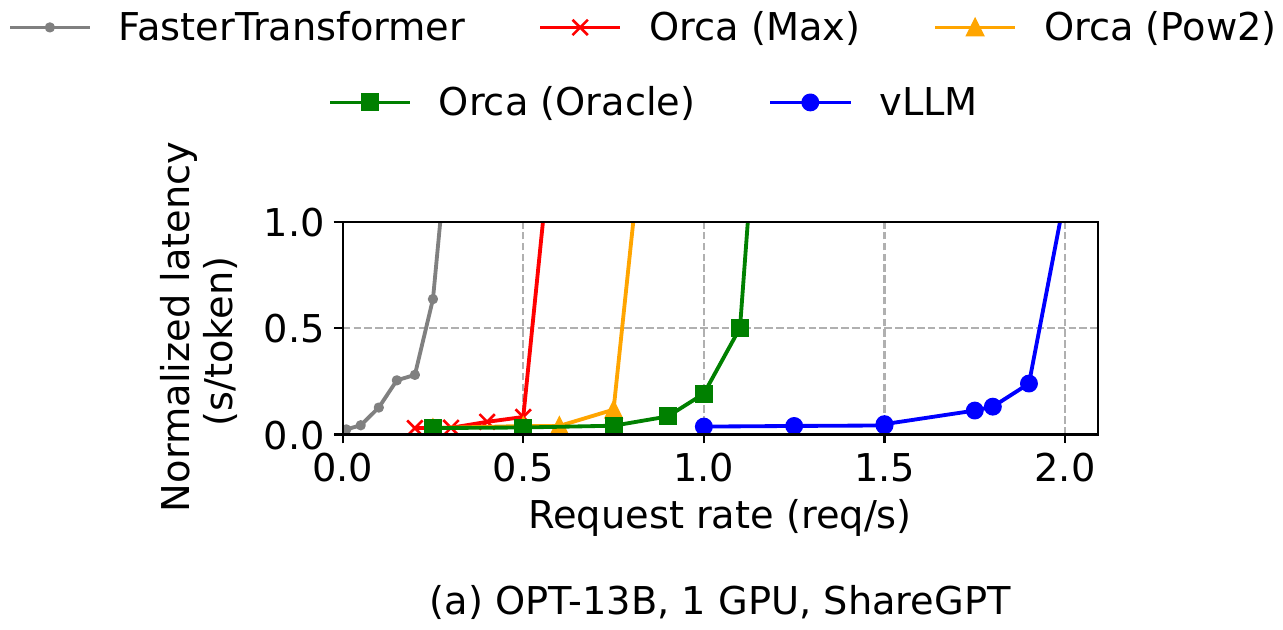
\includegraphics[width=\textwidth,height=5.3cm,keepaspectratio]{vllm_fig12a.png}
    \end{column}
    \begin{column}{0.36\textwidth}
      \small
      Each curve: latency per output token as the request rate grows. The knee is the load a server can sustain.\\[0.2cm]
      \textcolor{midgray}{\textbf{FasterTransformer}}: no iteration-level scheduling.\\[0.1cm]
      \textbf{Orca}: continuous batching; reserves contiguous cache.\\[0.1cm]
      \textbf{\textcolor{figmemory}{vLLM}}: continuous batching with a paged cache: \textbf{\val{vllm_rate_low} to \val{vllm_rate_high}$\times$} the rate of Orca (Oracle).
    \end{column}
  \end{columns}
  \mlsyscredit{Kwon et al., ``PagedAttention'' (vLLM), SOSP 2023, arXiv 2309.06180, Fig.~12a (OPT-13B, one A100, ShareGPT), cropped; legend rows rearranged.}
  \note{[1.5 min] The paper's own figure, cropped. Across: requests per second. Up: normalized latency, each request's end-to-end time divided by its output length. Every curve is flat until the server saturates, then the queue grows without bound. FasterTransformer forms a batch and runs it to completion; it saturates first. The three Orca curves use continuous batching but reserve contiguous cache (the next segment's problem); they move right in order of how little they over-reserve, Oracle knowing every length in advance. vLLM adds paging and sustains \val{vllm_rate_low} to \val{vllm_rate_high} times the request rate of Orca (Oracle) on ShareGPT, and up to \val{vllm_rate_ft} times FasterTransformer, at similar latency (the paper's numbers). ENGAGE: why does Orca (Oracle), which knows every answer's length, still saturate before vLLM? (Expected: it still reserves one contiguous region per request, so fragmentation limits the batch; segment 3.) WARN: these are Kwon et al.'s reimplementations of Orca, not the original system. FLEX: [OPTIONAL]; cutting it loses the measured knee.}
\end{frame}

\begin{frame}{Diagnose: why do all streams freeze at once?}
  \mlsysactivity{Diagnose}{1.5 min}
  \begin{columns}[c]
    \begin{column}{0.31\textwidth}
      \begin{mlsyscard}{errorstroke}\small
        TPOT is met most of the time, but now and then all streams pause at once.
      \end{mlsyscard}
      \vspace{0.12cm}
      {\footnotesize Measured (vLLM, H100, long prompts): ITL median \val{vb_itl_med_long} ms, p99 \textbf{\val{vb_itl_p99_long}} ms.}
    \end{column}
    \begin{column}{0.67\textwidth}
      \centering
      \mlsyssteps[width=\textwidth,height=4.4cm,keepaspectratio]{stall_step}{3}\\[0.08cm]
      \uncover<3->{\footnotesize Chunked: first token near \val{st_first} ms against \val{st_stall_ms}. Measured: \val{sarathi_low} to \val{sarathi_high}$\times$ the capacity of vLLM (Sarathi-Serve).}
    \end{column}
  \end{columns}
  \mlsyscredit{Derived from Model Serving, \S13.10.3 and \S13.9.4 (Llama 3 8B, \val{cs_w_gb} GB INT4 weights, \val{cs_ttft} ms per \val{cs_prompt}-token prefill at \val{prefill_eff}\% of peak, linear in tokens; \val{cs_tpot_target} ms TPOT). Agrawal et al., ``Sarathi-Serve,'' OSDI 2024, abstract.}
  \note{[3.5 min] [CORE] ENGAGE: one minute; what binds? Take answers before step 2. Step 1: Llama 3 8B, INT4 weights, one H100, \val{st_decodes} conversations decoding. Each step reads \val{cs_w_gb} GB of weights and \val{st_decodes} caches of \val{st_ctx} tokens, \val{st_bytes} GB: \val{st_dec_ms} ms, far under \val{cs_tpot_target} ms. Step 2: a \val{cs_prompt}-token prompt arrives, and continuous batching runs its prefill in the same step: \val{cs_ttft} plus \val{st_dec_ms}, \val{st_stall_ms} ms. All \val{st_decodes} streams wait \val{st_stall_ms} ms for their next token. This is the benchmark slide's p99 gap; Sarathi-Serve measured such generation stalls in vLLM. Step 3: split the prompt into \val{st_chunks} chunks of \val{st_chunk_tok} tokens, one per step: \val{st_chunk_pre} ms of prefill plus \val{st_dec_ms} ms, \val{st_chunk_ms} ms, under the target. The new request's first token comes after \val{st_chunks} steps, about \val{st_first} ms instead of \val{st_stall_ms}: chunking spends TTFT slack to protect TPOT. Measured: Sarathi-Serve served \val{sarathi_low} times more load on Mistral-7B and up to \val{sarathi_high} times on Yi-34B than vLLM under the same tail-latency limits. ENGAGE: what sets the largest safe chunk? (Expected: TPOT minus the decode step, over prefill time per token: \val{st_safe} tokens, derived; the chapter uses 512.) WARN: step times are derived floors. Land the segment: the TPOT target caps the batch; continuous batching fills it; chunking protects it.}
\end{frame}

% =============================================================================
% SECTION: CACHE BUDGET
% =============================================================================
\mlsysnote{[0.5 min] [CORE] Every newcomer needs memory for its cache. How many fit, and how much does the allocator waste?}
\mlsysdivider{How many chats fit in memory, and how much does allocation waste?}{Model Serving, \S13.9.4 (PagedAttention), \S13.9.5}
\section{Cache}

\begin{frame}{Estimate: how many 8K-token chats fit on one H100?}
  \mlsysactivity{Estimate}{2 min}
  \begin{columns}[T]
    \begin{column}{0.40\textwidth}
      \begin{mlsyscard}{mlsysaccent}
        \small\textbf{Given: Llama 3 8B, one H100}\\[0.1cm]
        \val{l3_kv_kb} KB per token (Lecture 6b)\\
        16-bit weights: \val{l3_w16_gb} of \val{h100_mem_gb} GB\\
        Conversation: \val{conv_tokens} tokens
      \end{mlsyscard}
      \small
      \uncover<2->{Per conversation: \val{conv_gb} GB\\[0.05cm]
      Free: $\val{h100_mem_gb} - \val{l3_w16_gb} = \val{free_gb}$ GB\\[0.05cm]
      About \textbf{\textcolor{mlsysaccent}{\val{n_conv} conversations}}}
    \end{column}
    \begin{column}{0.58\textwidth}
      \centering
      \only<1-2|handout:0>{}%
      \only<3|handout:0>{\safeimg[width=\textwidth,height=4.6cm,keepaspectratio]{kv_budget_8b.pdf}}%
      \only<4-|handout:1>{\safeimg[width=\textwidth,height=4.6cm,keepaspectratio]{kv_budget.pdf}}
    \end{column}
  \end{columns}
  \mlsyscredit{Model Serving, \S13.9.5 (Llama 3 8B, derived lines) and figure 8 (redrawn; \val{kv70_tok} B per token assumed for the 70B class). \val{h100_mem_gib} GB on the datasheet is \val{h100_mem_gb} GB in decimal units.}
  \note{[3.5 min] [CORE] ENGAGE: two minutes with a neighbor. Lecture 6b derived the \val{l3_kv_kb} KB per token for Llama 3.1 8B, which has Llama 3 8B's layers and heads and a longer window; take it as given. Step 2: an \val{conv_tokens}-token conversation holds \val{l3_kv_tok} bytes times \val{conv_tokens}, \val{conv_gb} GB. The weights leave \val{free_gb} GB, room for about \val{n_conv} conversations before any runtime workspace. The common error is forgetting the weights (\val{n_conv_noweights}). Step 3: the estimate as a picture. Each line is one batch size of Llama 3 8B conversations; the cache grows linearly with context, and \val{n_conv} conversations reach the \val{free_gb} GB budget at \val{conv_tokens} tokens (\val{n_conv} times \val{conv_gb} GB is \val{n_conv_gb} GB, derived). Step 4: a larger model, announced in the figure's title. A 70-billion-parameter-class model with 4-bit weights leaves \val{kv70_budget} GB for cache. Each token costs \val{kv70_ratio} times the 8B model's cache, so \val{kv70_batch} conversations fill the budget near \val{kv70_cross} tokens. The slope assumes \val{kv70_layers} layers and \val{kv70_heads} key-value heads of \val{kv70_hdim}, our assumption, which reproduces the chapter's crossing. Measured split from vLLM: a 13B model on a 40 GB A100 spends about \val{kwon_param_pct} percent of memory on weights and close to \val{kwon_kv_pct} percent on cache. WARN: memory caps how many conversations share each weight read; every extra thousand tokens of context costs conversations. FLEX: [CORE].}
\end{frame}

\begin{frame}{Reserving for the longest answer wastes most of the cache}
  \centering
  \mlsyssteps[width=0.92\textwidth,height=3.1cm,keepaspectratio]{frag_step}{3}\\[0.1cm]
  \uncover<4->{\safeimg[width=0.80\textwidth,height=2.7cm,keepaspectratio]{vllm_used.pdf}}
  \mlsyscredit{Diagram after Kwon et al., ``PagedAttention'' (vLLM), SOSP 2023, Fig.~3. Bars: Fig.~2 (OPT-13B, one A100, ShareGPT); Orca as reimplemented by Kwon et al.}
  \note{[2.5 min] [CORE] One strip of KV memory, in token slots. Step 1: a server that stores each cache in one contiguous region must reserve the maximum length up front, because it cannot know the answer's length. A has generated 70 tokens; the rest of its region is reserved for tokens that may never come. Step 2: B stops at 120 tokens, so 80 slots of its region are never used: internal fragmentation. Step 3: a finished request freed 100 slots, but a new 150-token request needs one contiguous range and cannot use the hole: external fragmentation, the chapter's example. Step 4: measured. The vLLM authors reimplemented Orca's allocator with three reservation policies; only \val{orca_used_low} to \val{orca_used_high} percent of the reserved memory held token states. Oracle even knows each answer's length in advance. vLLM, with paging, used \val{vllm_used} percent. The chapter states it as 60 to 80 percent wasted in naive implementations. ENGAGE: which waste would knowing every length in advance remove, and which would remain? (Expected: reservation; the external holes remain.) FLEX: [CORE].}
\end{frame}

\begin{frame}{Paging stores a growing cache in fixed blocks anywhere}
  \begin{columns}[c]
    \begin{column}{0.72\textwidth}
      \centering\mlsyssteps[width=\textwidth,height=5.6cm,keepaspectratio]{paging_step}{4}
    \end{column}
    \begin{column}{0.26\textwidth}
      \uncover<5->{\begin{mlsyscard}{GreenLine}\small\textbf{Measured, vLLM}\\[0.05cm]OPT-13B, one A100\\ batch \val{vllm_batch_orca} $\rightarrow$ \textbf{\val{vllm_batch_vllm}}\\ \val{vllm_batch_gain}$\times$\end{mlsyscard}}
    \end{column}
  \end{columns}
  \mlsyscredit{After Kwon et al., ``PagedAttention'' (vLLM), SOSP 2023, \S4.3 and Fig.~6 (block size 4 here; \val{block_default} by default). Bars: Fig.~13a, OPT-13B, ShareGPT.}
  \note{[3 min] [CORE] PagedAttention borrows the operating system's paging (first built on the Atlas computer, 1962). The cache lives in fixed-size blocks, and a block table maps each request's logical blocks to physical blocks anywhere in memory. Step 1: a 7-token prompt fills logical block 0 and three slots of block 1; the table maps them to physical blocks 7 and 1. One slot is free. Step 2: decode makes ``fathers''; it fills the free slot, and the table's count goes to 4. Step 3: the next token needs a new block; any free block will do, here 3. Step 4: request B's blocks interleave in the same pool. No region is reserved ahead, no hole is too small, and each sequence wastes at most its last, partly filled block. The attention kernel reads the blocks through the table directly. Step 5: measured: the average batch on the same GPU grew from \val{vllm_batch_orca} requests (Orca with Oracle) to \val{vllm_batch_vllm}, \val{vllm_batch_gain} times. ENGAGE: what happens to a request's blocks when it ends? (Expected: they return to the free pool for the next step.) WARN: paging decides where blocks live; the model decides how many a sequence needs. FLEX: [CORE].}
\end{frame}

\begin{frame}[t]{vLLM counts \val{log_conc} chats of \val{conv_tokens} tokens against our \val{n_conv}}
  \vspace{-0.25cm}\noindent{\footnotesize\textbf{The allocator:} a request gets blocks only as its tokens arrive}\par\vspace{0.05cm}
  \begin{logblock}[7]
    num\_required\_blocks = cdiv(num\_tokens, self.block\_size)\\
    num\_new\_blocks = num\_required\_blocks - len(req\_blocks)\\
    \textcolor{midgray}{[...]}\\
    \ind{4}new\_blocks = self.block\_pool.get\_new\_blocks(num\_new\_blocks)\\
    \ind{4}req\_blocks.extend(new\_blocks)
  \end{logblock}
  \vspace{0.08cm}
  {\footnotesize\textbf{The startup log:} Llama 3 8B, 16-bit, one H100, default settings}\par\vspace{0.05cm}
  \begin{logblock}[6.6]
    INFO 07-20 23:32:55 [gpu\_model\_runner.py:1624] Model loading took 14.9596 GiB and 0.153384 seconds\\
    INFO 07-20 23:32:56 [gpu\_worker.py:227] Available KV cache memory: 51.39 GiB\\
    INFO 07-20 23:32:56 [kv\_cache\_utils.py:715] GPU KV cache size: 420,976 tokens\\
    INFO 07-20 23:32:56 [kv\_cache\_utils.py:719] Maximum concurrency for 8,192 tokens per request: \textbf{\textcolor{errorstroke}{51.39x}}
  \end{logblock}
  \vspace{0.08cm}
  \uncover<2->{\footnotesize Estimate \val{n_conv} $\rightarrow$ \val{log_conc}: vLLM uses \val{log_util} of \val{h100_mem_gib} GiB and keeps \val{log_workspace_gib} GiB for activations (derived).}\\[0.05cm]
  \uncover<3->{\footnotesize Paged \val{log_req_tokens}-token chats: cdiv(\val{log_req_tokens}, \val{block_default}) $=$ \val{log_blocks} blocks; estimate \val{log_paged_est}, vLLM's pool \textbf{\val{log_paged_pool}} (derived).}
  \mlsyscredit{Code: vLLM v0.9.1 (b6553be), vllm/v1/core/single\_type\_kv\_cache\_manager.py, lines 121--127 (Apache 2.0). Log: github.com/vllm-project/vllm/issues/21266.}
  \note{[2.5 min] Two real artifacts. Top: vLLM's allocator, quoted from its source. A request needs the ceiling of its tokens over the block size, and only the difference from what it holds comes from the free pool. The code is the last slide's block table in five lines of Python. Bottom: a startup log posted in a public vLLM issue, the same model as our estimate, Llama 3 8B in 16-bit on one H100 with vLLM's defaults. The weights take \val{log_weights_gib} GiB, \val{log_weights_gb} GB, as the chapter says. The pool holds \val{log_tokens} tokens; at \val{l3_kv_tok} bytes each that is exactly the \val{log_kv_gib} GiB above, and \val{log_tokens} / \val{conv_tokens} = \val{log_conc} conversations (derived). Step 2: why not \val{n_conv}? vLLM claims \val{log_util_pct} percent of the GPU by default, \val{log_claimed_gib} GiB, and after the weights keeps \val{log_workspace_gib} GiB that its profiling run measured for activations (derived). The estimate ignored both and was \val{log_high_pct} percent high. Step 3: paged, a \val{log_req_tokens}-token conversation takes cdiv(\val{log_req_tokens}, \val{block_default}) = \val{log_blocks} blocks; the estimate's \val{free_gb} GB holds \val{log_paged_est}, vLLM's real pool \val{log_paged_pool} (derived). ENGAGE: which assumption would you fix first? (Expected: the memory cap and workspace; the bytes per token matched exactly.) FLEX: [OPTIONAL]; cutting it loses the allocator's own count; the chapter's own bound for 4-bit weights is about \val{cs_resident}.}
\end{frame}

\begin{frame}{Check: what does paging change, and what does it not?}
  \mlsysactivity{Vote}{2 min}
  \normalsize
  True or false?\\[0.3cm]
  \choice{1}{Paging reduces the cache bytes each token needs.}\uncover<2->{\enspace\textbf{\textcolor{errorstroke}{False}}}\\[0.25cm]
  \choice{2}{Two requests can share one system prompt's cache.}\uncover<2->{\enspace\textbf{\textcolor{GreenLine}{True}}}\\[0.25cm]
  \choice{3}{With paging, a sequence wastes at most one partly filled block.}\uncover<2->{\enspace\textbf{\textcolor{GreenLine}{True}}}\\[0.4cm]
  \uncover<2->{\small Paging decides where blocks live; the model decides how many bytes a token needs.}
  \mlsyscredit{Model Serving, \S13.9.4 and \S13.9.5; Kwon et al., SOSP 2023.}
  \note{[2 min] Peer instruction: vote on all three, one minute with a neighbor, vote again. Step 2: (1) false. The bytes per token come from the model: layers, key-value heads, head size, precision. Lecture 6b's levers (grouped-query attention, lower precision) change them; paging does not. (2) true. Two block tables can point at the same physical blocks; the next slide uses this. (3) true; about \val{block_waste_mb} MB for Llama 3 8B with \val{block_default}-token blocks. Students who say true to (1) confuse wasting less memory with needing less. The chapter's sentence to quote: paging decides where cache blocks live; it does not reduce how many blocks each sequence needs. FLEX: [OPTIONAL]; cutting it loses the paging vote.}
\end{frame}

\begin{frame}{Requests with a common prefix can share its cache blocks}
  \begin{columns}[c]
    \begin{column}{0.51\textwidth}
      \centering\mlsyssteps[width=\textwidth,height=3.4cm,keepaspectratio]{share_step}{2}
    \end{column}
    \begin{column}{0.47\textwidth}
      {\footnotesize\textbf{vLLM's cache settings} (vllm/config.py)}\par\vspace{0.05cm}
      \begin{logblock}[6.8]
        gpu\_memory\_utilization: float = 0.9\\
        enable\_prefix\_caching: Optional[bool] = None
      \end{logblock}
      \vspace{0.05cm}
      {\footnotesize Its docstring: ``Enabled by default for V1.''}
    \end{column}
  \end{columns}
  \vspace{0.1cm}
  \uncover<2->{\footnotesize Measured (vLLM): beam search (several candidate answers per prompt) shares blocks and saves \val{share_bs_low} to \val{share_bs_high}\% of KV memory.}\\[0.05cm]
  \uncover<2->{\footnotesize Overflow to host memory: reloading one \val{conv_tokens}-token cache over PCIe takes at least \val{reload_ms} ms, more than a \val{cs_tpot_target} ms TPOT (derived). The router sends a conversation's next turn to the replica that holds its cache.}
  \mlsyscredit{Model Serving, \S13.9.5, \S13.9.6, \S13.8.4 (reload \val{conv_gb} GB / \val{reload_gbps} GB/s, derived). Kwon et al., SOSP 2023, Fig.~15. Code: vLLM v0.9.1, vllm/config.py, CacheConfig, lines 1464 and 1487 (Apache 2.0).}
  \note{[2.5 min] [OPTIONAL] Step 1: many requests begin with the same \val{prefix_tokens}-token system prompt. Its cache, \val{prefix_mb} MB for Llama 3 8B, is stored once, and every block table points at the same blocks; a request that would write into a shared block first gets its own copy (copy on write). This is prefix caching. The code is vLLM's configuration. Prefix caching is on by default, and the \val{log_util} is the cap that cut the last slide's count from \val{n_conv} to \val{log_conc_0}. Step 2: \val{prefix_users} conversations sharing one copy save about \val{prefix_saved_gb} GB and skip \val{prefix_users_less1} times \val{prefix_tokens} tokens of prefill (derived). Measured in vLLM: sharing saved \val{share_ps_low} to \val{share_ps_high} percent of cache memory when sampling several answers to one prompt, and \val{share_bs_low} to \val{share_bs_high} percent in beam search. When the cache overflows, idle caches can move to host memory, but reloading one \val{conv_tokens}-token cache over PCIe takes at least \val{reload_ms} ms (derived), over a \val{cs_tpot_target} ms TPOT. Session affinity routes a conversation's next turn to the replica holding its cache. ENGAGE: why must the router know about the cache? (Expected: a turn sent elsewhere pays the prefill again.) Land the segment: free memory over each conversation's cache sets concurrency; paging and sharing give back what reservation wastes. FLEX: if cut, land the segment on the paging slide.}
\end{frame}

% =============================================================================
% SECTION: SPLITTING THE PHASES
% =============================================================================
\mlsysnote{[0.5 min] [CORE] Chunked prefill interleaved the two phases on one GPU. The other answer separates them. This segment comes from outside the chapter.}
\mlsysdivider{Should prefill and decode share an accelerator?}{Zhong et al., OSDI 2024 (DistServe); Patel et al., ISCA 2024 (Splitwise)}
\section{Splitting}

\begin{frame}{A GPU running both phases serves fewer requests than either alone}
  \begin{columns}[c]
    \begin{column}{0.62\textwidth}
      \centering\safeimg[width=\textwidth,height=3.6cm,keepaspectratio]{distserve_bars.pdf}
    \end{column}
    \begin{column}{0.36\textwidth}
      \centering\safeimg[width=\textwidth,height=2.4cm,keepaspectratio]{nvidia-a100.png}\\[0.08cm]
      {\footnotesize NVIDIA A100 (PCIe card shown). DistServe measured one 80 GB A100.}
    \end{column}
  \end{columns}
  \vspace{0.2cm}
  \centering{\small Goodput: requests/s that meet both TTFT and TPOT for \val{ds_slo_pct}\% of requests. \val{ds_in} tokens in, \val{ds_out} out.}
  \mlsyscredit{Zhong et al., ``DistServe,'' OSDI 2024, Fig.~1 and \S1 (\val{ds_params}B model, one 80 GB A100). Photo: Nvidia, CC BY-SA 4.0, Wikimedia Commons.}
  \note{[2.5 min] [CORE] The board in the photo is the measured device: one A100, the generation before the H100. Goodput is the rate of requests that meet both deadlines, here at \val{ds_slo_pct} percent attainment. DistServe measured a \val{ds_params}-billion-parameter model on one A100. Running both phases on one GPU, it sustains \val{ds_colo} requests per second. The same GPU doing only prefill sustains \val{ds_pre}; doing only decode, \val{ds_dec}. The phases interfere. A prefill stalls decode (the last segment), and decode steps delay the next prefill, so the colocated GPU must run lightly loaded to keep both deadlines. They also want different settings: prefill is efficient at small batches and benefits from splitting a layer across GPUs, while decode wants large batches. ENGAGE: if both phases fit on one GPU, why is the colocated number below both? (Expected: each phase's deadline is hurt by the other's work, so the GPU is kept far from full.) WARN: the three bars come from one experiment; a different model or prompt length shifts them. FLEX: [CORE].}
\end{frame}

\begin{frame}{Estimate: how many prefill GPUs per decode GPU?}
  \mlsysactivity{Estimate}{2 min}
  \begin{columns}[c]
    \begin{column}{0.44\textwidth}
      \begin{mlsyscard}{mlsysaccent}
        \small\textbf{Given (measured, per A100)}\\[0.1cm]
        Prefill only: \val{ds_pre} requests/s\\
        Decode only: \val{ds_dec} requests/s\\
        Both phases: \val{ds_colo} requests/s
      \end{mlsyscard}
      \small
      \uncover<2->{One decode GPU: \val{ds_dec}/s\\[0.05cm]
      Prefill: $\val{ds_dec} / \val{ds_pre} = \val{ds_pre_exact} \rightarrow$ \val{ds_pre_n} GPUs\\[0.05cm]
      $\val{ds_dec} / \val{ds_gpus} = \val{ds_per_gpu}$ per GPU: \textbf{\textcolor{mlsysaccent}{\val{ds_gain}$\times$}} of \val{ds_colo}}
    \end{column}
    \begin{column}{0.54\textwidth}
      \centering\uncover<2->{\safeimg[width=\textwidth,height=4.5cm,keepaspectratio]{distserve_pool.pdf}}
    \end{column}
  \end{columns}
  \mlsyscredit{Zhong et al., ``DistServe,'' OSDI 2024, \S1 and Fig.~1.}
  \note{[2.5 min] ENGAGE: two minutes; size the two pools so neither waits on the other. Step 2: one decode GPU handles \val{ds_dec} requests per second; prefill GPUs at \val{ds_pre} each need \val{ds_dec} divided by \val{ds_pre}, \val{ds_pre_exact}, so \val{ds_pre_n}. \Val{ds_gpus_word} GPUs serve \val{ds_dec} requests per second, \val{ds_per_gpu} each, \val{ds_gain} times the colocated \val{ds_colo}. The prefill GPUs send each request's cache to the decode GPU. This is disaggregation: separate pools, each sized and batched for its own phase. DistServe reports up to \val{ds_more} times more requests than vLLM under the same deadlines, or deadlines \val{ds_tighter} times tighter. WARN: students who answer 1:1 give the decode GPU idle time; students who answer 3:1 buy prefill capacity that sits idle. The ratio depends on prompt and answer lengths; a long-document workload needs more prefill. FLEX: [OPTIONAL]; cutting it loses the prefill-to-decode ratio.}
\end{frame}

\begin{frame}{Splitting costs one cache transfer and frees the hardware choice}
  \begin{columns}[c]
    \begin{column}{0.54\textwidth}
      \centering\safeimg[width=\textwidth,height=3.2cm,keepaspectratio]{split_link.pdf}\\[0.1cm]
      {\footnotesize \val{ds_kv_gb} GB per \val{ds_in}-token OPT-66B request. Measured transfer: under \val{ds_xfer_pct}\% of latency (DistServe); \val{sw_xfer_pct}\% of the request, about \val{sw_xfer_ms} ms on H100 (Splitwise).}
    \end{column}
    \begin{column}{0.43\textwidth}
      \uncover<2->{\begin{mlsyscard}{mlsysaccent}\small
        \textbf{Measured, Splitwise:}\\[0.05cm]
        Capping a GPU from \val{sw_cap_from} to \val{sw_cap_to} W barely slows decode.\\[0.05cm]
        Split clusters: \textbf{\val{sw_gain}$\times$} the throughput at \textbf{\val{sw_cost_pct}\%} lower cost.
      \end{mlsyscard}}
    \end{column}
  \end{columns}
  \mlsyscredit{Zhong et al., ``DistServe,'' OSDI 2024, \S3.3 and \S6.3. Patel et al., ``Splitwise,'' ISCA 2024, \S III-F, \S VI-A, Figs.~8 and 9, abstract.}
  \note{[2.5 min] [OPTIONAL] Step 1: the price of splitting is moving each request's cache from a prefill GPU to a decode GPU. For OPT-66B a \val{ds_in}-token prompt has \val{ds_kv_gb} GB of cache; at \val{ds_kv_rate} requests per second that is \val{ds_traffic} GB/s, about \val{ds_traffic_gbps} Gbps, small against the \val{ds_link} GB/s of NVLink between GPUs in one node. Measured: DistServe's transfer was under \val{ds_xfer_pct} percent of total latency for OPT-175B; Splitwise measured \val{sw_xfer_pct} percent of the request, about \val{sw_xfer_ms} ms on H100, by sending each layer's cache while the next layer computes. Step 2: once separate, each pool can use a different chip. Decode is bound by memory bandwidth, so Splitwise found that capping a GPU's power from \val{sw_cap_from} to \val{sw_cap_to} W barely slows it, and its decode power stays flat as the batch grows. Its clusters gave \val{sw_gain} times the throughput at \val{sw_cost_pct} percent lower cost. ENGAGE: chunked prefill or disaggregation for a single 8-GPU server? (Expected: both are used; chunking needs no transfer, splitting needs a fast link.) LINK: a model too large for one GPU is split across a node's GPUs by tensor parallelism (\S13.9.5); no lecture in this course teaches it, so point students to that section. Volume I stops at one machine. Land the segment aloud.}
\end{frame}

% =============================================================================
% SECTION: PER TOKEN
% =============================================================================
\mlsysnote{[0.5 min] [CORE] Every lever so far changed how many conversations share each step. That sharing also sets the price of a token.}
\mlsysdivider{What does one token cost in joules and dollars?}{Model Serving, \S13.9.6 (Napkin Math 13.5), \S13.10.3}
\section{Per Token}

\begin{frame}{Joules per token fall as the batch fills}
  \centering
  \safeimg[width=0.92\textwidth,height=3.8cm,keepaspectratio]{joules_token.pdf}\\[0.2cm]
  {\small Measured (Splitwise): decode power does not rise with the batch, so the token rate sets the joules.}\\[0.15cm]
  \uncover<2->{\small Google, May 2024 to May 2025: \textbf{\textcolor{mlsysaccent}{\val{g_reduction}$\times$}} less energy per median prompt, \val{g_util}$\times$ of it from utilization.}
  \mlsyscredit{Derived: \val{p_node_kw} kW node and \val{p_low} W at low use (Model Serving, Napkin Math 13.5) over the token rates of \S13.9.2. Patel et al., ``Splitwise,'' Fig.~8. Elsworth et al., arXiv 2508.15734, 2025.}
  \note{[2 min] [OPTIONAL] Step 1: a node draws about \val{p_node} W (GPU plus host share) whether a step carries one sequence or \val{batch_32}. Over the GPT-2 XL rates: \val{p_node} W / \val{rate_1} tokens/s = \val{j1} J per token at batch 1; \val{p_node} / \val{rate_32} = \val{j32} J at batch \val{batch_32}. The gray bar uses the chapter's power for a poorly used node, \val{p_low_gpu} W GPU plus \val{p_host} W host: \val{p_low} / \val{rate_1} = \val{j1_low} J. All derived. Even at \val{p_low} W, batch 1 costs \val{j_low_ratio} times batch \val{batch_32}: power changes at most \val{p_ratio} times while the token rate changes \val{rate_growth} times, and Splitwise measured decode power flat with batch. LINK: the chapter's Napkin Math 13.5, \val{cc_joules} J against \val{cc_low_joules} J per token, is the same mechanism: a tenth of the token rate, with power falling only from \val{p_node} to \val{p_low} W. Step 2: Google's median Gemini text prompt used \val{g_reduction} times less energy after one year, \val{g_model} times from models and \val{g_util} times from busier machines; \val{g_wh} Wh per prompt, counting host, idle reserve, and facility. WARN: the \val{g_reduction} times is a whole-service number. LINK: Lecture 15b owns carbon and lifecycle accounting. ENGAGE: a reasoning model writes 2,000 hidden tokens before answering; what happens to energy per question? (Expected: it grows with every token.) FLEX: [OPTIONAL].}
\end{frame}

\begin{frame}{Estimate: what does a million tokens cost on one H100?}
  \mlsysactivity{Estimate}{2 min}
  \begin{columns}[c]
    \begin{column}{0.40\textwidth}
      \begin{mlsyscard}{mlsysaccent}
        \small\textbf{Given: Llama 3 8B}\\[0.05cm]
        4-bit weights; H100, \$\val{cs_price}/hour\\
        Prefill (assumed): \val{cs_req_rate} requests/s\\
        \val{cs_prompt} + \val{cs_decode} tokens each
      \end{mlsyscard}
      \small
      \uncover<2->{$\val{cs_req_rate} \times 3{,}600 \times \text{\val{cs_tokens}}$\\ $= \val{cs_mtok_h}$M tokens/hour\\[0.1cm]
      $\$\val{cs_price} / \val{cs_mtok_h} = \mathbf{\textcolor{mlsysaccent}{\$\val{cs_usd_m}}}$ per million\\[0.05cm]
      {\footnotesize\textcolor{midgray}{A case-study bound, unmeasured.}}}
    \end{column}
    \begin{column}{0.58\textwidth}
      \centering
      \only<1-2|handout:0>{\safeimg[width=\textwidth,height=5.1cm,keepaspectratio]{api_price_step1.pdf}}%
      \only<3-|handout:1>{\safeimg[width=\textwidth,height=5.1cm,keepaspectratio]{api_price_step2.pdf}}
    \end{column}
  \end{columns}
  \mlsyscredit{Model Serving, \S13.10.3 and Checkpoint 13.6. Prices: figure 9, redrawn from its MLSysIM series (vendor list prices per million input tokens, historical).}
  \note{[2.5 min] [CORE] ENGAGE: two minutes. The chapter's case study rents one H100 for about \$\val{cs_price} an hour and assumes prefill admits \val{cs_prefill_rate} prompt tokens per second, \val{cs_req_rate} requests per second of \val{cs_prompt}-token prompts; prefill is the limit that binds here, ahead of memory. Step 2: each request counts its prompt and its \val{cs_decode} generated tokens, \val{cs_tokens} in all, so \val{cs_mtok_h} million tokens an hour, \$\val{cs_usd_m} per million tokens. The plot is the book's figure of public API list prices per million input tokens, 2023 to 2025, on a log scale: \$\val{price_gpt4} for the original GPT-4 down to \$\val{price_flash} for Gemini 1.5 Flash. Step 3: the green line is the case study's floor. WARN: the \$\val{cs_usd_m} is a bound for one workload; Checkpoint 13.6 requires a load test that records TTFT and TPOT distributions and the completed request rate, and the price then counts only requests that met both deadlines. The plotted prices are for input tokens only, and list prices also include margin, larger models, and idle capacity. ENGAGE: which price points lie near the floor, and what does that say about those providers' batches? FLEX: [CORE].}
\end{frame}

% =============================================================================
% CLOSE
% =============================================================================
\begin{frame}{Why \val{llama_int_tpot} ms keeps fewer tokens than \val{llama_conv_tpot} ms}
  \mlsysactivity{Retrieval}{1.5 min}
  \begin{columns}[c]
    \begin{column}{0.41\textwidth}
      \centering\safeimg[width=\textwidth,height=1.6cm,keepaspectratio]{thumb_hook_thumb.pdf}\\[0.02cm]
      {\footnotesize Offline \val{llama_off};\ \val{llama_conv_tpot} ms: \val{llama_conv};\ \val{llama_int_tpot} ms: \val{llama_int} tokens/s}\\[0.1cm]
      \uncover<2->{\footnotesize Streams in decode $\le$ tokens/s $\times$ TPOT\\[0.05cm]
      $\text{\val{llama_conv}} \times \val{llama_conv_tpot_s}$: at most $\mathbf{\text{\val{streams_200}}}$\\ $\text{\val{llama_int}} \times \val{llama_int_tpot_s}$: at most $\mathbf{\val{streams_40}}$\\[0.03cm]
      {\footnotesize\textcolor{midgray}{(derived bounds)}}}
    \end{column}
    \begin{column}{0.57\textwidth}\small
      \only<1|handout:0>{\normalsize Name the three limits on how many sequences share a decode step, and one lever for each.}%
      \only<2->{\small Memory: \val{syn_free_gb} GB $/$ \val{syn_conv_mb} MB $=$ \textbf{\val{syn_streams}} streams\\
      {\footnotesize\textcolor{midgray}{(derived; 16-bit weights and cache; \val{cs_tokens} tokens assumed)}}\\[0.05cm]
      \textbf{\textcolor{mlsysaccent}{\val{llama_conv_tpot} ms: memory binds.\quad \val{llama_int_tpot} ms: the deadline binds.}}\\[0.15cm]}
      \uncover<3->{\small
      \begin{tabular}{@{}P{1.5cm}P{5.6cm}@{}}\toprule
        \textbf{Limit} & \textbf{Levers} \\\midrule
        TPOT & speculative decoding; fewer weight bytes \\[0.05cm]
        Memory & paging; prefix sharing \\[0.05cm]
        Prompts & chunked prefill; disaggregation \\\bottomrule
      \end{tabular}}
    \end{column}
  \end{columns}
  \mlsyscredit{MLPerf Inference v5.0, 5.0-0020 (Llama 2 70B, \val{mlperf_gpus}$\times$ H100). Little 1961, as in Part 1.}
  \note{[4 min] [CORE] Back to the hook. Step 1: retrieval, 90 seconds. Step 2: Little's law from Part 1: streams decoding at once equal tokens per second times TPOT. At most \val{llama_conv} times \val{llama_conv_tpot_s} = \val{streams_200} streams under \val{llama_conv_tpot} ms; \val{llama_int} times \val{llama_int_tpot_s} = \val{streams_40} under \val{llama_int_tpot} ms (derived bounds). Eight H100s hold \val{mlperf_gpus} times \val{h100_mem_gb} = \val{syn_mem_gb} GB; 16-bit Llama 2 70B weights take about \val{syn_w16_gb} GB (\val{syn_w_ratio} times the chapter's \val{syn_w4_gb} GB at 4 bits), leaving \val{syn_free_gb} GB. A \val{cs_tokens}-token conversation (the case study's length, assumed) at \val{kv70_tok} bytes per token holds \val{syn_conv_mb} MB, so memory fits \val{syn_free_gb} GB / \val{syn_conv_mb} MB = \val{syn_streams} streams. Under \val{llama_conv_tpot} ms memory binds, and the deadline has slack: \val{syn_streams} / \val{llama_conv} is a \val{syn_step_ms} ms step. That is why the conversational run keeps \val{llama_conv_pct} percent. Under \val{llama_int_tpot} ms only \val{streams_40} fit the deadline, so the deadline binds and throughput falls to \val{llama_int_pct} percent. WARN: with 8-bit weights and cache, memory holds about \val{syn8_streams} (\val{syn8_free_gb} GB / \val{syn8_conv_mb} MB), still under \val{streams_200}. Step 3: read the table; each lever moves one limit. ENGAGE: which lever first on the \val{llama_int_tpot} ms server? (Expected: one that shortens the step, since the deadline binds.) WARN: serving \val{llama_conv} tokens/s under \val{llama_int_tpot} ms takes about \val{syn_servers} times the servers (\val{llama_conv} / \val{llama_int}, derived). FLEX: [CORE].}
\end{frame}

\begin{frame}{Takeaways}
  \thumbline{thumb_phases_step4.pdf}{Prefill sets TTFT with arithmetic; decode sets TPOT with one weight read per step.}\\[0.12cm]
  \thumbline{thumb_frontier_step3.pdf}{Each sequence adds its cache read to the step, so a TPOT target caps the batch.}\\[0.12cm]
  \thumbline{thumb_cb_step7.pdf}{Continuous batching fills a freed slot at the next step; chunking keeps prompts from stalling it.}\\[0.12cm]
  \thumbline{thumb_kv_budget_8b.pdf}{Free memory over cache per conversation sets concurrency (\val{n_conv} estimated, \val{log_conc} in vLLM's log); paging and sharing recover it.}\\[0.12cm]
  \thumbline{thumb_joules_token.pdf}{Joules and dollars per token follow how full each decode step runs.}
  \note{[1.5 min] [CORE] One line per idea. Ask students which slide taught each line. If short on time, read the second and the fourth.}
\end{frame}

\begin{frame}{Open questions}
  \begin{columns}[c]
    \begin{column}{0.65\textwidth}
      \small
      \begin{itemize}\setlength{\itemsep}{0.12cm}
        \item Reasoning models choose to spend more tokens per question. Each costs decode time, cache memory, and joules. Where should a service cap that spending, and who sets the cap?
        \item Prices per token fell by orders of magnitude in two years, and energy per prompt fell \val{g_reduction}$\times$ in one. Will total serving energy fall or rise?
        \item Decode runs well on power-capped or older accelerators. Should chip makers build chips for one phase only?
      \end{itemize}
    \end{column}
    \begin{column}{0.33\textwidth}
      \centering\mlsysphoto[width=\textwidth,height=3.4cm,keepaspectratio]{datacenters-ashburn-aerial.jpg}\\[0.08cm]
      {\footnotesize Data centers and their electrical substations in Ashburn, Virginia}
    \end{column}
  \end{columns}
  \mlsyscredit{Photo: Theodore Christopher, CC0, Wikimedia Commons.}
  \note{[1.5 min] [OPTIONAL] No single answer. Pick one for discussion or assign one as a short written response. The first comes from Systems Perspective 13.7. The second is Jevons paradox (\S13.10): cheaper steam power raised total coal use in the nineteenth century; cheaper inference may raise total demand. The third follows from Splitwise's power measurements and DistServe's separate pools.}
\end{frame}

\begin{frame}{Read and explore}
  \small
  \begin{itemize}\setlength{\itemsep}{0.02cm}
    \item \textbf{Read:} Model Serving, \S13.9 and \S13.10.3; Checkpoints 13.5 and 13.6; Napkin Math 13.5 and equation 15 by hand.
    \item Yu et al., ``Orca,'' OSDI 2022: iteration-level scheduling.
    \item Kwon et al., ``PagedAttention'' (vLLM), SOSP 2023: the block table.
    \item Agrawal et al., ``Sarathi-Serve,'' OSDI 2024: chunked prefill.
    \item Zhong et al., ``DistServe,'' OSDI 2024: separate prefill and decode pools.
    \item Patel et al., ``Splitwise,'' ISCA 2024: latency, batching, and power by phase.
  \end{itemize}
  \note{[1 min] [CORE] The chapter first, with the self-check questions for \S13.9 and \S13.10. Orca is the origin of continuous batching. Kwon et al. measure the cache waste and design the block table. Sarathi-Serve measures generation stalls and chunked prefill. DistServe sizes separate prefill and decode pools. Splitwise measures latency, batching, and power by phase on A100 and H100 servers. FLEX: add the lab your course uses for serving.}
\end{frame}

\begin{frame}[c]
  \begin{columns}[c]
    \begin{column}{0.34\textwidth}
      \centering\mlsyskitfig[width=\textwidth,height=4.2cm,keepaspectratio]{stack_operations}
    \end{column}
    \begin{column}{0.62\textwidth}
      {\small\textcolor{lightgray}{NEXT LECTURE \textbar{} ML OPERATIONS, PART 1}}\\[0.5cm]
      {\LARGE\bfseries The service is up and fast. How do we know it is still right?}
    \end{column}
  \end{columns}
  \note{[1 min] [CORE] Two lectures kept the service fast. Lecture 14 asks whether it stays correct. One example to leave with: if the server resizes images with a different library than training did, or swaps the color channel order, every latency dashboard stays green while predictions change (training-serving skew, \S13.8.5).}
\end{frame}

\end{document}
